\chapter{\IfLanguageName{dutch}{Draaien backend in Docker containers}{Running backend in Docker containers}}
\label{ch:docker-backend}

Na het opsplitsen van de backend in drie afzonderlijke services, zijn ze vervolgens gecontaineriseerd door ze elk in een aparte Docker-container te plaatsen. Deze containerisatie -aanpak biedt een gestandaardiseerde en geïsoleerde omgeving voor het uitvoeren van de services.

Elke backend-service wordt nu uitgevoerd in zijn eigen Docker-container, waardoor ze volledig geïsoleerd zijn van elkaar en van andere delen van het systeem.

Voor elke service wordt een Dockerfile gemaakt om de configuratie van de respectieve containers te definiëren. Deze Dockerfiles bevatten instructies voor het bouwen van de containers, het installeren van de benodigde afhankelijkheden en het starten van de services.

Voor de Node.js code werd bijvoorbeeld een Dockerfile opgesteld die begint met het gebruik van de officiële Node.js 20-image als basis. Vervolgens worden de benodigde bestanden gekopieerd naar de werkomgeving binnen de container, dependencies geïnstalleerd met npm en de applicatie gestart met het juiste commando.

Voor de Python code werd een vergelijkbare Dockerfile gemaakt, die begint met het gebruik van de officiële Python 3.12-image als basis. Vervolgens worden de benodigde bestanden gekopieerd, dependencies geïnstalleerd met pip en de applicatie gestart met het juiste commando.

Met deze Dockerfiles kunnen de backend-services eenvoudig worden gebouwd en gedistribueerd als Docker-containers, waardoor een consistente en gecontroleerde uitvoeringsomgeving wordt gegarandeerd, ongeacht het onderliggende hostsysteem. Dit draagt bij aan een naadloze implementatie en schaalbaarheid van de applicatie in diverse omgevingen.

Met het \texttt{docker run -dp 127.0.0.1:****:9080} commando kan de container worden gestart en kan de service worden benaderd via de opgegeven poort. Op deze manier kunnen de services lokaal worden uitgevoerd en getest, voordat ze worden geïntegreerd in de bredere applicatie-architectuur.

In figuur \ref{fig:getUserDocker} is te zien hoe de gebruikersgegevens worden opgehaald uit de MongoDB-database in een Docker-container op poort ****.

\begin{figure}[H]
	\centering	
	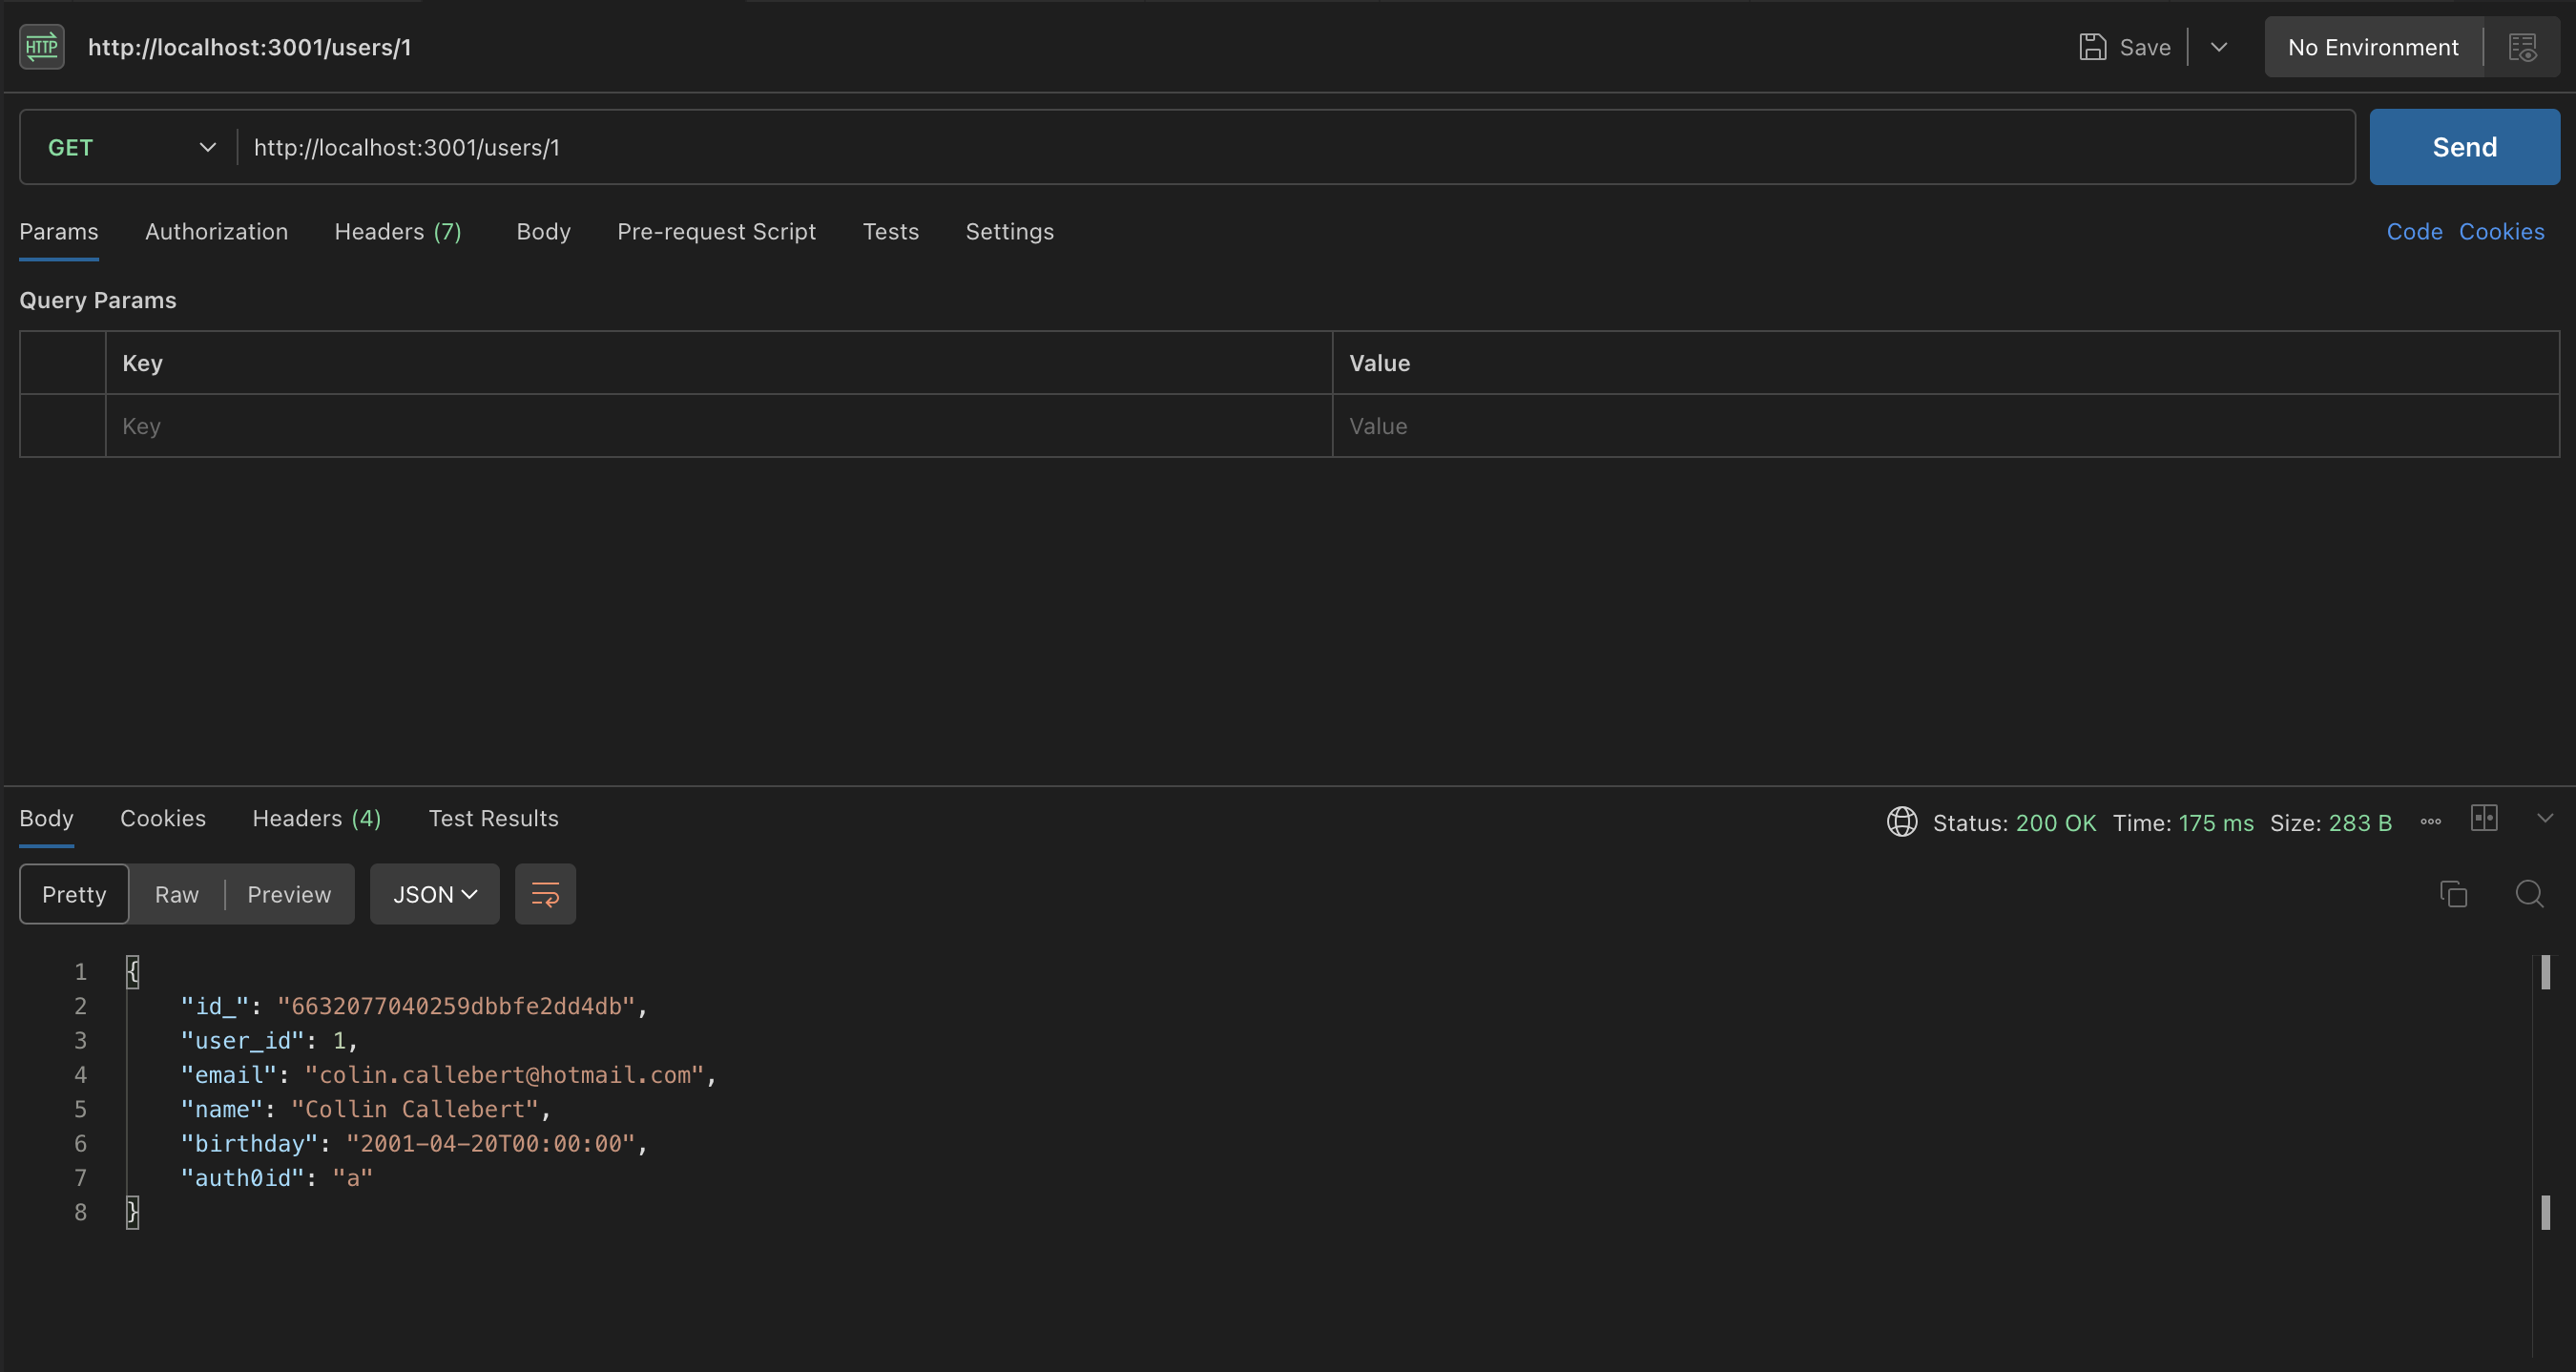
\includegraphics[width = 16cm]{getUseDocker.png} 
	\caption{Haal gebruikersgegevens op uit de MongoDB- database in een Docker-container}
	\label{fig:getUserDocker} 
\end{figure}
\FloatBarrier